\documentclass[oneside,10pt]{article}

%%%%%%%%%%%%%
%Mise en page
%%%%%%%%%%%%%
%\usepackage[margin=0cm,papersize={5.5cm,5cm}]{geometry}
%%max: \usepackage[margin=0cm,papersize={16cm,24cm}]{geometry}
\usepackage{nopageno}

%%%%%%%%%%%%%
%Pour les graphiques
%%%%%%%%%%%%%
\usepackage{tikz}
\usetikzlibrary{arrows,external,calc,positioning,intersections}
%\tikzexternalize[prefix=tikz/,only named=true]
\tikzexternalize[only named=true]
% rajouter " -shell-escape"  la commande pdflatex ou xelatex
% l'option "only named=true" fait en sorte que seulement les figures avec un nom sont externalises
% Pour definir le nom de l'image :
% \tikzsetnextfilename{<file_name>}}

%\usetikzlibrary{arrows,calc,positioning,intersections}
%%%\tikzexternalize[prefix=tikz/,only named=true]
%%\tikzexternalize[only named=true]
%%% rajouter " -shell-escape"  la commande pdflatex ou xelatex
%%% l'option "only named=true" fait en sorte que seulement les figures avec un nom sont externalises
%%% Pour definir le nom de l'image :
%%% \tikzsetnextfilename{<file_name>}}

% pour avoir dash-dot
  \tikzset{
    dash-dot/.style={
    dash pattern=on 4pt off 3pt on 1pt off 3pt,
  },
  }
% pour avoir dash-dot-dot
  \tikzset{
    dash-dot-dot/.style={
    dash pattern=on 4pt off 3pt on 1pt off 3pt on 1pt off 3pt,
  },
  }

\usepackage{pgfplots}
\usetikzlibrary{pgfplots.groupplots}
	% Pour que ce soit compatible avec la version 1.6
	\pgfplotsset{compat=1.6}
	% pour les label des axes
	\pgfplotsset{tick scale binop={\times}}
%	% le style de la légende  
%	\pgfplotsset{every axis legend/.append style={
%		at={(0.9,0.9)},
%		anchor=north east}}
%	% pour avoir un espace separant les mille
	\pgfkeys{/pgf/number format/.cd,fixed,
		precision=4,
		%use comma, %pour utiliser la virgule
		set thousands separator={\,}}
%	% position des label sur x et y
%	\pgfplotsset{every axis x label/.style=
%		{at={(ticklabel cs:0.5)},anchor=near ticklabel}}
%	\pgfplotsset{every axis y label/.style=
%		{at={(ticklabel cs:0.5)},anchor=near ticklabel}}
%	% Modifier les marks
%	\pgfplotsset{every mark/.append style={solid}}
	% pour augmenter la taille des lignes
	\pgfplotsset{every axis/.append style={
		line width=1pt,
		axis line style={line width=0.4pt},
		tick style={line width=0.4pt}}}

\definecolor{LHSVLightBlue}{cmyk}{0.99,0.29,0.00,0.12}
\definecolor{LHSVDarkBlue}{cmyk}{1.00,0.35,0.00,0.20}
\definecolor{EdfBlue}{RGB}{0,91,187}
\definecolor{EdfDBlue}{RGB}{9,53,122}
\definecolor{EdfLBlue}{RGB}{56,174,255}
\definecolor{EdfOrange}{RGB}{255,160,47}
\definecolor{EdfLOrange}{RGB}{243,157,0}
\definecolor{EdfGreen}{RGB}{80,158,47}
\definecolor{EdfDGreen}{RGB}{196,214,47}
\definecolor{PantoneRed}{RGB}{232,17,45}
\definecolor{PantonePurple}{RGB}{137,79,191}
\definecolor{PantoneGreen}{RGB}{0,153,124}
\definecolor{PantonePink}{RGB}{214,2,112}



%%%%%%%%%%%%%%
%%Options de codes
%%%%%%%%%%%%%%
%\usepackage{xfrac}
\usepackage{xifthen}
\usepackage{calculator}


%%%%%%%%%%%%%
%Pour les équations
%%%%%%%%%%%%%
\usepackage{bm} %pour avoir des symbol en gras quand ils ne sont pas dfini dans mathbf
\renewcommand{\vec}[1]{\bm{#1}}

%------------------------------------
\begin{document}
%------------------------------------

%------------------------------------
\section{Experimental setup}
%------------------------------------

%\tikzset{external/force remake=true}
\tikzsetnextfilename{CanalAlgExpSetup}

\begin{tikzpicture}[baseline]%[xscale=0.02,yscale=10]%baseline, fait en sorte que les graphiques soit aligné
  \begin{axis}[
% Position des axes
  axis x line=none,axis y line=none,clip=false,
%  x dir=reverse,
% largeur du graphiques
  width=0.9\textwidth,height=0.245\textheight,scale only axis,
  %height=0.5\textwidth,
% max et min
  xmin=-3,xmax=6,ymin=-0.25,ymax=2.2
%  xmin=-0.2,xmax=0.2,ymin=-0.5,ymax=1
  ]
    % Les remplisages solides
    \shade[inner color=white,outer color=gray] (axis cs:0.05,0.4) rectangle (axis cs:-0.05,0.5);
    %
    \shade[inner color=gray,outer color=white] (axis cs:-0.1,-0.05) rectangle (axis cs:0,0.05);
    \fill[color=white] (axis cs:-0.05,0) rectangle (axis cs:-0.1,0.05);
    \shade[bottom color=white,top color=gray] (axis cs:-2,-0.05) rectangle (axis cs:-0.05,0);
    \shade[left color=gray,right color=white] (axis cs:-0.05,0) rectangle (axis cs:0,0.45);
    %
    \shade[inner color=gray,outer color=white] (axis cs:0.1,-0.05) rectangle (axis cs:0,0.05);
    \fill[color=white] (axis cs:0.05,0) rectangle (axis cs:0.1,0.05);
    \shade[bottom color=white,top color=gray] (axis cs:0.05,-0.05) rectangle (axis cs:5,0);
    \shade[left color=white,right color=gray] (axis cs:0.05,0) rectangle (axis cs:0,0.45);
    %
    \shade[bottom color=gray,top color=white] (axis cs:-2,2) rectangle (axis cs:5,2.05);
    % Les bords solides
    \draw (axis cs:-2,2) -- (axis cs:5,2);
    \draw (axis cs:-2,0) -- (axis cs:-0.05,0) -- (axis cs:-0.05,0.5) -- (axis cs:0.05,0.5) -- (axis cs:0.05,0)  -- (axis cs:5,0);
    % Débit entrant
    \draw [->,thick] (axis cs:-2.5,0.02) -- (axis cs:-2.05,0.02);
    \draw [->,thick] (axis cs:-2.5,0.4) -- (axis cs:-2.05,0.4);
    \draw [->,thick] (axis cs:-2.5,0.8) -- (axis cs:-2.05,0.8);
    \draw [->,thick] (axis cs:-2.5,1.2) -- (axis cs:-2.05,1.2);
    \draw [->,thick] (axis cs:-2.5,1.6) -- (axis cs:-2.05,1.6);
    \draw [->,thick] (axis cs:-2.5,1.98) -- (axis cs:-2.05,1.98);
    \draw [thick] (axis cs:-2.5,0.02) -- (axis cs:-2.5,1.98);
    % Dimensions
    \draw[<->] (axis cs:-1,0) -- (axis cs:-1,1) node[inner sep=2mm,shape=rectangle,fill=white]{\small $2$ m} -- (axis cs:-1,2);
    %
    \draw (axis cs:-0.05,0.51) -- (axis cs:-0.05,0.75);
    \draw[->] (axis cs:-0.15,0.725) -- (axis cs:-0.05,0.725);
    \draw (axis cs:0.05,0.51) -- (axis cs:0.05,0.75);
    \draw[->] (axis cs:0.15,0.725) -- (axis cs:0.05,0.725);
    \draw (axis cs:0,0.82) node[inner sep=0mm,shape=rectangle]{\small $0.1$ m};
    %
    \draw (axis cs:0.06,0.5) -- (axis cs:0.55,0.5);
    \draw[<->] (axis cs:0.5,0) -- (axis cs:0.5,0.25) node[inner sep=2mm,shape=rectangle,fill=white]{\small $0.5$ m} -- (axis cs:0.5,0.5);
    %
    \draw (axis cs:-2.5,2.05) node[inner sep=0mm,shape=rectangle]{\small $0.5$ m/s};
    %
    \draw (axis cs:5,1) node[inner sep=0mm,shape=rectangle,text width=1.5cm,font=\small,text centered]{%$\genfrac{}{}{0pt}{0}{\text{imposed depth}}{\text{of 0.3 m}}$
    imposed depth of $0.3$ m on the outflow boundary};
    %
    \draw (axis cs:-2.5,1) node[inner sep=2mm,shape=rectangle,anchor=east,text width=1.7cm,font=\small,text centered]{Inflow with constant depth of $0.3$ m};
    %
    % Axis
    \draw[->,thick,shorten >=0pt,shorten <=0pt] (axis cs:-2.3,-0.2) -- (axis cs:-2.3,-0.05) node[shape=rectangle,anchor=north east]{\small y};
    \draw[->,thick,shorten >=0pt,shorten <=0pt] (axis cs:-2.3,-0.2) -- (axis cs:-2.05,-0.2) node[shape=rectangle,anchor=west]{\small x};
  \end{axis}
\end{tikzpicture}%


%------------------------------------
\section{Fluid velocities}
%------------------------------------

%\tikzset{external/force remake=true}
\tikzsetnextfilename{CanalAlgFluidVelocities}

\begin{tikzpicture}[baseline]%[xscale=0.02,yscale=10]%baseline, fait en sorte que les graphiques soit aligné
  \begin{axis}[
	%Name
	name=AlgCanalFluidVel,
% Pour avoir les axes en dessus
  enlargelimits=false,axis on top=true,clip=false,
% titres des axes
  xlabel=$x$ (m),ylabel=$y$ (m),
  xtick={-2,0,1,2,3,4,5},%xmajorgrids,
% Position des axes
%  axis x line=none,axis y line=none,
%  x dir=reverse,
% largeur du graphiques
  width=0.9\textwidth,height=0.245\textheight,scale only axis,
  %height=0.5\textwidth,
% max et min
  xmin=-3,xmax=6.5,ymin=0,ymax=2
%  xmin=-0.2,xmax=0.2,ymin=-0.5,ymax=1
  ]
    % Clipping
     \clip (axis cs:-3,-0.2) rectangle (axis cs:6.5,2.2);
    % Les remplisages solides
    \shade[inner color=white,outer color=gray] (axis cs:0.05,0.4) rectangle (axis cs:-0.05,0.5);
    %
    \shade[inner color=gray,outer color=white] (axis cs:-0.1,-0.05) rectangle (axis cs:0,0.05);
    \fill[color=white] (axis cs:-0.05,0) rectangle (axis cs:-0.1,0.05);
    \shade[bottom color=white,top color=gray] (axis cs:-3,-0.05) rectangle (axis cs:-0.05,0);
    \shade[left color=gray,right color=white] (axis cs:-0.05,0) rectangle (axis cs:0,0.45);
    %
    \shade[inner color=gray,outer color=white] (axis cs:0.1,-0.05) rectangle (axis cs:0,0.05);
    \fill[color=white] (axis cs:0.05,0) rectangle (axis cs:0.1,0.05);
    \shade[bottom color=white,top color=gray] (axis cs:0.05,-0.05) rectangle (axis cs:7,0);
    \shade[left color=white,right color=gray] (axis cs:0.05,0) rectangle (axis cs:0,0.45);
    %
    \shade[bottom color=gray,top color=white] (axis cs:-3,2) rectangle (axis cs:7,2.05);
    % Les bords solides
    \draw (axis cs:-3,2) -- (axis cs:7,2);
    \draw (axis cs:-3,0) -- (axis cs:-0.05,0) -- (axis cs:-0.05,0.5) -- (axis cs:0.05,0.5) -- (axis cs:0.05,0)  -- (axis cs:5,0);
    % Les profils
%    \addplot[color=black] table[x=u_plus_x_1_tel,y=y_1_tel ] {./Courbes/prof_cour_tel.res};
%    \label{plot:prof_vit_tel}
    \addplot[mark=o,only marks] table[x=u_plus_x_1_exp,y=y_1_exp ] {./Courbes/prof_cour_exp.res};
    \label{plot:prof_vit_exp}
    \addplot[color=black,style=dashed] table[x=u_plus_x_1_of,y=y_1_of ] {./Courbes/prof_cour_of.res};
    \label{plot:prof_vit_of}
    %
    \addplot[color=black] table[x=u_plus_x_1_tel,y=y_1_tel ] {./Courbes/profils_cour_tel_v6p3.txt};
    \label{plot:prof_vit_tel_v6p3}
    %
    \addplot[color=EdfBlue,dashed,line width=2pt] table[x=u_plus_x_1_tel,y=y_1_tel ] {../../profils_cour_tel.txt};
    \label{plot:prof_vit_tel}
    %
    \foreach \i in {2,...,7} {
%      \addplot[color=black] table[x=u_plus_x_\i_tel,y=y_\i_tel ] {./Courbes/prof_cour_tel.res};
      \addplot[mark=o,only marks] table[x=u_plus_x_\i_exp,y=y_\i_exp ] {./Courbes/prof_cour_exp.res};
      \addplot[color=black,style=dashed] table[x=u_plus_x_\i_of,y=y_\i_of ] {./Courbes/prof_cour_of.res};
      %
      \addplot[color=black] table[x=u_plus_x_\i_tel,y=y_\i_tel ] {./Courbes/profils_cour_tel_v6p3.txt};
      %
      \addplot[color=EdfBlue,dashed,line width=2pt] table[x=u_plus_x_\i_tel,y=y_\i_tel ] {../../profils_cour_tel.txt};
      %
    }
    % les axes des vitesses
%    \draw (axis cs:-2.5,2) node[inner sep=2mm,anchor=south]{$\left|U\right|$};
    \addplot[black!70!white,nodes near coords,point meta=explicit symbolic,font=\footnotesize,inner sep=1mm,anchor=south east] 
             coordinates {(-2.5,0)[$U_x$ (m/s)]};
    \foreach \x in {-2,0,1,2,3,4,5} {
      \addplot[black!70!white,mark=|,only marks,mark size={2pt}] coordinates {(\x,0) (\x+0.5,0) };
      \addplot[black!70!white,mark=|,only marks,mark size={1pt}] coordinates {(\x+0.25,0) (\x+0.75,0) };
      \addplot[black!70!white,->,overlay] coordinates {(\x,0) (\x+0.85,0) };
      \foreach \y in {0,0.5} {
        \addplot[black!70!white,nodes near coords,point meta=\y,font=\tiny] coordinates {(\x+\y,0)[]};
%        \addplot[black!70!white,nodes near coords,point meta=explicit symbolic,font=\tiny] coordinates {(\x+\y,0)[\y]};
      }
    }    
  \end{axis}
  % Legend
  \draw[thick] ($(AlgCanalFluidVel.south west)+(0pt,-1.5cm)+(0pt,+2pt)$) circle(2pt) ++ (10pt,0pt) circle(2pt) ++ (10pt,0pt) circle(2pt) ++(5pt,0pt) node[anchor=west] {Experimental results};
  \draw[thick,dashed] ($(AlgCanalFluidVel.south west)+(0pt,-2cm)+(0pt,+2pt)$) -- ++ (20pt,0pt) ++(5pt,0pt) node[anchor=west] {Numerical results from OpenFoam};
  \draw[thick] ($(AlgCanalFluidVel.south west)+(0pt,-2.5cm)+(0pt,+2pt)$) -- ++ (20pt,0pt) ++(5pt,0pt) node[anchor=west] {Numerical results from version 6.3};
  \draw[thick,draw=EdfBlue,dashed,line width=2pt] ($(AlgCanalFluidVel.south west)+(0pt,-3.0cm)+(0pt,+2pt)$) -- ++ (20pt,0pt) ++(5pt,0pt) node[anchor=west] {Numerical results from current version};
\end{tikzpicture}%



%------------------------------------
\section{Experimental set up for particle measurement}
%------------------------------------

%\tikzset{external/force remake=true}
\tikzsetnextfilename{CanalAlgExpSetup2}

\begin{tikzpicture}[baseline]
		\begin{groupplot}[
    		group style={
        	group name=my plots,
        	group size=2 by 1,
        	%xlabels at=edge bottom,
        	%xticklabels at=edge bottom,
			%x descriptions at=edge bottom,
        	%vertical sep=0pt,
        	horizontal sep=10pt,
    		},
% Position des axes
  axis x line=bottom,axis y line=none,clip=false,
%  x dir=reverse,
% titres des axes
  xlabel=$x (m)$,
  xtick={-1.05,-0.05,0.225,1.225,1.4,2.4},%xmajorgrids,
  x tick label style={font=\tiny,rotate=60},
% largeur du graphiques
  width=0.45\linewidth,height=0.3375\linewidth,scale only axis,
  %height=0.5\textwidth,
% max et min
%  xmin=-0.2,xmax=0.2,ymin=-0.5,ymax=1
  ]
  \nextgroupplot[xmin=-1.5,xmax=3,ymin=-0.25,ymax=2]
    % Les remplisages solides
    \shade[inner color=white,outer color=gray] (axis cs:0.05,0.4) rectangle (axis cs:-0.05,0.5);
    %
    \shade[inner color=gray,outer color=white] (axis cs:-0.1,-0.05) rectangle (axis cs:0,0.05);
    \fill[color=white] (axis cs:-0.05,0) rectangle (axis cs:-0.1,0.05);
    \shade[bottom color=white,top color=gray] (axis cs:-1.5,-0.05) rectangle (axis cs:-0.05,0);
    \shade[left color=gray,right color=white] (axis cs:-0.05,0) rectangle (axis cs:0,0.45);
    %
    \shade[inner color=gray,outer color=white] (axis cs:0.1,-0.05) rectangle (axis cs:0,0.05);
    \fill[color=white] (axis cs:0.05,0) rectangle (axis cs:0.1,0.05);
    \shade[bottom color=white,top color=gray] (axis cs:0.05,-0.05) rectangle (axis cs:3,0);
    \shade[left color=white,right color=gray] (axis cs:0.05,0) rectangle (axis cs:0,0.45);
    % Les bords solides
    \draw (axis cs:-1.5,0) -- (axis cs:-0.05,0) -- (axis cs:-0.05,0.5) -- (axis cs:0.05,0.5) -- (axis cs:0.05,0)  -- (axis cs:3,0);
    % la surface libre
    \draw (axis cs:-1.5,0.3) -- (axis cs:-0.05,0.3);
    \draw[smooth] (axis cs:3,0.3) -- (axis cs:0.1,0.26)-- (axis cs:0.05,0.28);
    %Les fenêtres de mesure
    \draw[fill=white,thick] (axis cs:-0.05,0.29) rectangle (axis cs:-1.05,0.33);
    \draw (axis cs:-0.55,0.33) node[anchor=south,font=\tiny,]{Window 1};
    %
    \draw[fill=white,thick,dash pattern=on 3pt off 2pt] (axis cs:1.225,0.26) rectangle (axis cs:0.225,0.30);
    \draw (axis cs:0.725,0.30) node[anchor=south,font=\tiny,]{Window 2};
    %
    \draw[fill=white,thick,dash pattern=on 3pt off 2pt] (axis cs:2.4,0.28) rectangle (axis cs:1.4,0.32);
    \draw (axis cs:1.9,0.32) node[anchor=south,font=\tiny,]{Window 3};
    % La camera
    \draw (axis cs:-0.5,1.8) rectangle (axis cs:-0.6,1.6);
    \draw[fill=black] (axis cs:-0.52,1.6) rectangle (axis cs:-0.58,1.55);
    \draw (axis cs:-0.6,1.7) node[inner sep=2mm,shape=rectangle,anchor=west,text width=1.5cm,font=\tiny]{Camera};
    % Particule
    \draw[fill=black] (axis cs:-1.4,0.2) circle (1pt);
    \addplot[smooth] coordinates{(-1.4,0.2) (-1.2,0.17) (-1.1,0.22) (-1.0,0.21)};
    \draw[->,shorten >=0pt,shorten <=0pt] (axis cs:-1.005,0.22) -- (axis cs:-0.985,0.22);
    % further annotations
    %\draw[<-] (axis cs:-1.6,0.3) -- (axis cs:-1.8,0.4) node[inner sep=0mm,shape=rectangle,font=\tiny,anchor=south]{Particle};
    \draw[] (axis cs:-1.5,0.2) node[inner sep=0mm,shape=rectangle,font=\tiny,anchor=east]{Particle};
    \draw[<-] (axis cs:-0.2,0.33) -- (axis cs:-0.4,0.9) node[inner sep=2mm,shape=rectangle,font=\tiny]{Plexiglas surface};
    % Axis
    \draw[->,thick,shorten >=0pt,shorten <=0pt] (axis cs:-1.4,0.8) -- (axis cs:-1.4,1.05) node[shape=rectangle,anchor=north east]{\small z};
    \draw[->,thick,shorten >=0pt,shorten <=0pt] (axis cs:-1.4,0.8) -- (axis cs:-1.15,0.8) node[shape=rectangle,anchor=west]{\small x};
%
%  \nextgroupplot[xmin=-1.5,xmax=3,ymin=-0.25,ymax=2]
%    % Les remplisages solides
%    \shade[inner color=white,outer color=gray] (axis cs:0.05,0.4) rectangle (axis cs:-0.05,0.5);
  \nextgroupplot[axis x line=none,axis y line=none,clip=false,xmin=0,xmax=1,ymin=0,ymax=1]
    \addplot graphics [xmin=0,xmax=1,ymin=0,ymax=1] {./Images/Photocanal1_052_bw};
  \end{groupplot}
  % legend
  \draw ($(my plots c1r1.south)+(0pt,-1.7cm)$) node[anchor=north] {(a) Schematic diagram (side view)};
  \draw ($(my plots c2r1.south)+(0pt,-1.7cm)$) node[anchor=north] {(b) Photograph};
\end{tikzpicture}%


%------------------------------------
\section{Explanation of the figures}
%------------------------------------

%\tikzset{external/force remake=true}
\tikzsetnextfilename{CanalAlgAnnotatedFigure}

\begin{tikzpicture}[baseline]%[xscale=0.02,yscale=10]%baseline, fait en sorte que les graphiques soit aligné
  \begin{axis}[
% Pour avoir les axes en dessus
  enlargelimits=false,axis on top=true,clip=false,
% titres des axes
  xlabel=$x$ (m),ylabel=$y$ (m),
  %xtick={-2,0,1,2,3,4,5},%xmajorgrids,
% Position des axes
%  axis x line=none,axis y line=none,
%  x dir=reverse,
% largeur du graphiques
  width=\linewidth,height=0.75\linewidth,%scale only axis,
  %height=0.5\textwidth,
% max et min
%  xmin=-1.5,xmax=0.1,ymin=0,ymax=1.5
  xmin=-0.5,xmax=1.5,ymin=0,ymax=1.5
  ]
    % Les remplisages solides
    \shade[inner color=white,outer color=gray] (axis cs:0.05,0.4) rectangle (axis cs:-0.05,0.5);
    %
    \shade[inner color=gray,outer color=white] (axis cs:-0.1,-0.05) rectangle (axis cs:0,0.05);
    \fill[color=white] (axis cs:-0.05,0) rectangle (axis cs:-0.1,0.05);
    \shade[bottom color=white,top color=gray] (axis cs:-0.5,-0.05) rectangle (axis cs:-0.05,0);
    \shade[left color=gray,right color=white] (axis cs:-0.05,0) rectangle (axis cs:0,0.45);
    %
    \shade[inner color=gray,outer color=white] (axis cs:0.1,-0.05) rectangle (axis cs:0,0.05);
    \fill[color=white] (axis cs:0.05,0) rectangle (axis cs:0.1,0.05);
    \shade[bottom color=white,top color=gray] (axis cs:0.05,-0.05) rectangle (axis cs:1.5,0);
    \shade[left color=white,right color=gray] (axis cs:0.05,0) rectangle (axis cs:0,0.45);
    %
    %\shade[bottom color=gray,top color=white] (axis cs:-1.5,2) rectangle (axis cs:0.1,2.05);
    % Les bords solides
    %\draw (axis cs:-1.5,2) -- (axis cs:3.5,2);
    \draw (axis cs:-0.5,0) -- (axis cs:-0.05,0) -- (axis cs:-0.05,0.5) -- (axis cs:0.05,0.5) -- (axis cs:0.05,0)  -- (axis cs:1.5,0);
%%%%%%%%%%%%%%%%%%%%%%%%%%%%%%%%%%%%%%%%%%%%%%%%%%%%%%%%%%%%%%%%%%
    % L'échelle
    \draw[color=black!30!] (axis cs:0.725,0.5) -- (axis cs:1.225,1);
    \draw[color=black!30!] (axis cs:0.975,0.75) -- ($(axis cs:0.975,0.75)!3pt!90:(axis cs:1.225,1)$);
    \draw[color=black!30!] (axis cs:0.975,0.75) -- ($(axis cs:0.975,0.75)!3pt!-90:(axis cs:1.225,1)$);
    \draw[color=black!30!] (axis cs:1.225,1) -- ($(axis cs:1.225,1)!3pt!90:(axis cs:0.975,0.75)$);
    \draw[color=black!30!] (axis cs:1.225,1) -- ($(axis cs:1.225,1)!3pt!-90:(axis cs:0.975,0.75)$);
    \path (axis cs:0.725,0.5) -- (axis cs:1.225,1)
          node[pos=0.5,sloped,above] {\small\color{black!70!}0.25}
          node[pos=1,sloped,above] {\small\color{black!70!}0.5}
          ;
    \draw[color=black!30!] (axis cs:0.725,0.5) -- (axis cs:0.225,1);
    \draw[color=black!30!] (axis cs:0.475,0.75) -- ($(axis cs:0.475,0.75)!3pt!90:(axis cs:0.225,1)$);
    \draw[color=black!30!] (axis cs:0.475,0.75) -- ($(axis cs:0.475,0.75)!3pt!-90:(axis cs:0.225,1)$);
    \draw[color=black!30!] (axis cs:0.225,1) -- ($(axis cs:0.225,1)!3pt!90:(axis cs:0.475,0.75)$);
    \draw[color=black!30!] (axis cs:0.225,1) -- ($(axis cs:0.225,1)!3pt!-90:(axis cs:0.475,0.75)$);
    \path (axis cs:0.725,0.5) -- (axis cs:0.225,1)
          node[pos=0.5,sloped,above] {\small\color{black!70!}0.25}
          node[pos=1,sloped,above] {\small\color{black!70!}0.5}
          ;
    \draw[color=black!30!] (axis cs:0.725,0.5) -- (axis cs:1.225,0);
    \draw[color=black!30!] (axis cs:0.975,0.25) -- ($(axis cs:0.975,0.25)!3pt!90:(axis cs:1.225,0)$);
    \draw[color=black!30!] (axis cs:0.975,0.25) -- ($(axis cs:0.975,0.25)!3pt!-90:(axis cs:1.225,0)$);
    \draw[color=black!30!] (axis cs:1.225,0) -- ($(axis cs:1.225,0)!3pt!90:(axis cs:0.975,0.25)$);
    \draw[color=black!30!] (axis cs:1.225,0) -- ($(axis cs:1.225,0)!3pt!-90:(axis cs:0.975,0.25)$);
    \path (axis cs:0.725,0.5) -- (axis cs:1.225,0)
          node[pos=0.5,sloped,above] {\small\color{black!70!}0.25}
          node[pos=1,sloped,above] {\small\color{black!70!}0.5}
          ;
    \draw[color=black!30!] (axis cs:0.725,0.5) -- (axis cs:0.225,0);
    \draw[color=black!30!] (axis cs:0.475,0.25) -- ($(axis cs:0.475,0.25)!3pt!90:(axis cs:0.225,0)$);
    \draw[color=black!30!] (axis cs:0.475,0.25) -- ($(axis cs:0.475,0.25)!3pt!-90:(axis cs:0.225,0)$);
    \draw[color=black!30!] (axis cs:0.225,0) -- ($(axis cs:0.225,0)!3pt!90:(axis cs:0.475,0.25)$);
    \draw[color=black!30!] (axis cs:0.225,0) -- ($(axis cs:0.225,0)!3pt!-90:(axis cs:0.475,0.25)$);
    \path (axis cs:0.725,0.5) -- (axis cs:0.225,0)
          node[pos=0.5,sloped,above] {\small\color{black!70!}0.25}
          node[pos=1,sloped,above] {\small\color{black!70!}0.5}
          ;
    % Le point de relachement
    \addplot[mark=*,only marks,color=black,fill=black] table[x=x_rel,y=y_rel] {./Courbes/mesure2_lache2_exp.txt};
    % Les contours
    \addplot[color=black] table[x=x_decoup,y=y_decoup] {./Courbes/mesure2_lache2_exp.txt};
    \addplot[color=black,thick,fill=black,fill opacity=0.2] table[x=x_np_exp,y=y_np_exp] {./Courbes/mesure2_lache2_exp.txt};
    \addplot[color=black,thick,dashed,fill=black,fill opacity=0.2] table[x=x_np_of,y=y_np_of] {./Courbes/mesure2_lache2_of.txt};
    \addplot[color=black,thick,dotted,fill=black,fill opacity=0.2] table[x=x_np,y=y_np] {./Courbes/mesure2_lache2_v6p3.txt};
%%%%%%%%%%%%%%%%%%%%%%%%%%%%%%%%%%%%%%%%%%%%%%%%%%%%%%%%%%%%%%%%%%
    % Annotations
    \node[inner sep=2mm,shape=rectangle,text width=2cm,font=\small,anchor=north,text centered]   (wind_measur)  at (axis cs:0.4,1.4)
    	{Window of measurement};   
    \draw[->] (wind_measur.south) -- (axis cs:0.45,1.01);
    \node[inner sep=2mm,shape=rectangle,text width=1.3cm,font=\small,anchor=north,text centered]   (injec_poin)  at (axis cs:-0.25,0.5)
    	{Particle injection point};   
    \draw[->] (injec_poin.east) -- (axis cs:0.15,0.44);
    \node[inner sep=2mm,shape=rectangle,text width=2cm,font=\small,anchor=west,text centered]   (scale)  at (axis cs:1.6,0.15)
    	{Axis for the proportion of particles in this quadrant};   
    \draw[->] (scale.west) -- (axis cs:1.13,0.11);
    \node[inner sep=2mm,shape=rectangle,text width=1.5cm,font=\small,anchor=west,text centered]   (4_quadrants)  at (axis cs:1.55,0.75)
    	{The four quadrants};
    \draw[->] (4_quadrants.west) -- (axis cs:0.6,0.95);
    \draw[->] (4_quadrants.west) -- (axis cs:0.6,0.2);
    \draw[->] (4_quadrants.west) -- (axis cs:1.1,0.9);
    \draw[->] (4_quadrants.west) -- (axis cs:1.1,0.4);
    \node[inner sep=2mm,shape=rectangle,text width=3cm,font=\small,text centered,]   (measurement)  at (axis cs:-0.15,0.85)
    	{A shaded zone linking the proportion of particles present in each quadrant};
    \draw[->] (measurement.east) -- (axis cs:0.45,0.75);
  \end{axis} 
\end{tikzpicture}%


%------------------------------------
\section{Results: Proportion of particles}
%------------------------------------


\tikzset{external/force remake=true}
\tikzsetnextfilename{CanalAlgQuadrantNpart}

\begin{tikzpicture}[baseline]%[xscale=0.02,yscale=10]%baseline, fait en sorte que les graphiques soit aligné
  \begin{axis}[
	%Name
	name=AlgCanalNpart,
% Pour avoir les axes en dessus
  enlargelimits=false,axis on top=true,clip=false,
% titres des axes
  xlabel=$x$ (m),ylabel=$y$ (m),
  %xtick={-2,0,1,2,3,4,5},%xmajorgrids,
% Position des axes
%  axis x line=none,axis y line=none,
%  x dir=reverse,
% largeur du graphiques
  width=\linewidth,height=0.5\linewidth,%scale only axis,
  %height=0.5\textwidth,
% max et min
%  xmin=-1.5,xmax=0.1,ymin=0,ymax=1.5
  xmin=-0.5,xmax=1.5,ymin=0,ymax=1.5
  ]
    % Les remplisages solides
    \shade[inner color=white,outer color=gray] (axis cs:0.05,0.4) rectangle (axis cs:-0.05,0.5);
    %
    \shade[inner color=gray,outer color=white] (axis cs:-0.1,-0.05) rectangle (axis cs:0,0.05);
    \fill[color=white] (axis cs:-0.05,0) rectangle (axis cs:-0.1,0.05);
    \shade[bottom color=white,top color=gray] (axis cs:-0.5,-0.05) rectangle (axis cs:-0.05,0);
    \shade[left color=gray,right color=white] (axis cs:-0.05,0) rectangle (axis cs:0,0.45);
    %
    \shade[inner color=gray,outer color=white] (axis cs:0.1,-0.05) rectangle (axis cs:0,0.05);
    \fill[color=white] (axis cs:0.05,0) rectangle (axis cs:0.1,0.05);
    \shade[bottom color=white,top color=gray] (axis cs:0.05,-0.05) rectangle (axis cs:1.5,0);
    \shade[left color=white,right color=gray] (axis cs:0.05,0) rectangle (axis cs:0,0.45);
    %
    %\shade[bottom color=gray,top color=white] (axis cs:-1.5,2) rectangle (axis cs:0.1,2.05);
    % Les bords solides
    %\draw (axis cs:-1.5,2) -- (axis cs:3.5,2);
    \draw (axis cs:-0.5,0) -- (axis cs:-0.05,0) -- (axis cs:-0.05,0.5) -- (axis cs:0.05,0.5) -- (axis cs:0.05,0)  -- (axis cs:1.5,0);
%%%%%%%%%%%%%%%%%%%%%%%%%%%%%%%%%%%%%%%%%%%%%%%%%%%%%%%%%%%%%%%%%%
    % L'échelle
    \draw[color=black!30!] (axis cs:0.725,0.5) -- (axis cs:1.225,1);
    \draw[color=black!30!] (axis cs:0.975,0.75) -- ($(axis cs:0.975,0.75)!3pt!90:(axis cs:1.225,1)$);
    \draw[color=black!30!] (axis cs:0.975,0.75) -- ($(axis cs:0.975,0.75)!3pt!-90:(axis cs:1.225,1)$);
    \draw[color=black!30!] (axis cs:1.225,1) -- ($(axis cs:1.225,1)!3pt!90:(axis cs:0.975,0.75)$);
    \draw[color=black!30!] (axis cs:1.225,1) -- ($(axis cs:1.225,1)!3pt!-90:(axis cs:0.975,0.75)$);
    \path (axis cs:0.725,0.5) -- (axis cs:1.225,1)
          node[pos=0.5,sloped,above] {\small\color{black!70!}0.25}
          node[pos=1,sloped,above] {\small\color{black!70!}0.5}
          ;
    \draw[color=black!30!] (axis cs:0.725,0.5) -- (axis cs:0.225,1);
    \draw[color=black!30!] (axis cs:0.475,0.75) -- ($(axis cs:0.475,0.75)!3pt!90:(axis cs:0.225,1)$);
    \draw[color=black!30!] (axis cs:0.475,0.75) -- ($(axis cs:0.475,0.75)!3pt!-90:(axis cs:0.225,1)$);
    \draw[color=black!30!] (axis cs:0.225,1) -- ($(axis cs:0.225,1)!3pt!90:(axis cs:0.475,0.75)$);
    \draw[color=black!30!] (axis cs:0.225,1) -- ($(axis cs:0.225,1)!3pt!-90:(axis cs:0.475,0.75)$);
    \path (axis cs:0.725,0.5) -- (axis cs:0.225,1)
          node[pos=0.5,sloped,above] {\small\color{black!70!}0.25}
          node[pos=1,sloped,above] {\small\color{black!70!}0.5}
          ;
    \draw[color=black!30!] (axis cs:0.725,0.5) -- (axis cs:1.225,0);
    \draw[color=black!30!] (axis cs:0.975,0.25) -- ($(axis cs:0.975,0.25)!3pt!90:(axis cs:1.225,0)$);
    \draw[color=black!30!] (axis cs:0.975,0.25) -- ($(axis cs:0.975,0.25)!3pt!-90:(axis cs:1.225,0)$);
    \draw[color=black!30!] (axis cs:1.225,0) -- ($(axis cs:1.225,0)!3pt!90:(axis cs:0.975,0.25)$);
    \draw[color=black!30!] (axis cs:1.225,0) -- ($(axis cs:1.225,0)!3pt!-90:(axis cs:0.975,0.25)$);
    \path (axis cs:0.725,0.5) -- (axis cs:1.225,0)
          node[pos=0.5,sloped,above] {\small\color{black!70!}0.25}
          node[pos=1,sloped,above] {\small\color{black!70!}0.5}
          ;
    \draw[color=black!30!] (axis cs:0.725,0.5) -- (axis cs:0.225,0);
    \draw[color=black!30!] (axis cs:0.475,0.25) -- ($(axis cs:0.475,0.25)!3pt!90:(axis cs:0.225,0)$);
    \draw[color=black!30!] (axis cs:0.475,0.25) -- ($(axis cs:0.475,0.25)!3pt!-90:(axis cs:0.225,0)$);
    \draw[color=black!30!] (axis cs:0.225,0) -- ($(axis cs:0.225,0)!3pt!90:(axis cs:0.475,0.25)$);
    \draw[color=black!30!] (axis cs:0.225,0) -- ($(axis cs:0.225,0)!3pt!-90:(axis cs:0.475,0.25)$);
    \path (axis cs:0.725,0.5) -- (axis cs:0.225,0)
          node[pos=0.5,sloped,above] {\small\color{black!70!}0.25}
          node[pos=1,sloped,above] {\small\color{black!70!}0.5}
          ;
    % Le point de relachement
    \addplot[mark=*,only marks,color=black,fill=black] table[x=x_rel,y=y_rel] {./Courbes/mesure2_lache2_exp.txt};
    % Les contours
    \addplot[color=black] table[x=x_decoup,y=y_decoup] {./Courbes/mesure2_lache2_exp.txt};
    % Les resultats
    \addplot[color=black,thick,fill=black,fill opacity=0.2] table[x=x_np_exp,y=y_np_exp] {./Courbes/mesure2_lache2_exp.txt};
    \addplot[color=black,thick,dashed,fill=black,fill opacity=0.2] table[x=x_np_of,y=y_np_of] {./Courbes/mesure2_lache2_of.txt};
    \addplot[color=black,thick,dotted,fill=black,fill opacity=0.2] table[x=x_np,y=y_np] {./Courbes/mesure2_lache2_v6p3.txt};
    \addplot[color=EdfBlue,thick,fill=EdfBlue,fill opacity=0.2] table[x=x_np,y=y_np] {../../mesure2_lache2_Tel2D.txt};
  \end{axis}
  % Legend
  \draw[color=black,thick,fill=black,fill opacity=0.2] ($(AlgCanalNpart.south west)+(0pt,-1.5cm)+(0pt,-5pt)$) rectangle ++(20pt,10pt) ++(5pt,-6.5pt) node[anchor=west,opacity=1] {Experimental results};
  \draw[color=black,thick,dashed,fill=black,fill opacity=0.2] ($(AlgCanalNpart.south)+(-0.5cm,-1.5cm)+(0pt,-5pt)$) rectangle ++(20pt,10pt) ++(5pt,-6.5pt) node[anchor=west,opacity=1] {OpenFoam results};
  \draw[color=black,thick,dotted,fill=black,fill opacity=0.2] ($(AlgCanalNpart.south west)+(0pt,-2.5cm)+(0pt,-5pt)$) rectangle ++(20pt,10pt) ++(5pt,-6.5pt) node[anchor=west,opacity=1] {TELEMAC-2D 6.3};
  \draw[color=EdfBlue,thick,fill=EdfBlue,fill opacity=0.2] ($(AlgCanalNpart.south)+(-0.5cm,-2.5cm)+(0pt,-5pt)$) rectangle ++(20pt,10pt) ++(5pt,-6.5pt) node[anchor=west,opacity=1,color=black] {TELEMAC-2D current version};
\end{tikzpicture}%

%------------------------------------
\section{Results: Mean time of residence}
%------------------------------------


\tikzset{external/force remake=true}
\tikzsetnextfilename{CanalAlgQuadrantTrsd}


\begin{tikzpicture}[baseline]%[xscale=0.02,yscale=10]%baseline, fait en sorte que les graphiques soit aligné
  \begin{axis}[
	%Name
	name=AlgCanalTrsd,
% Pour avoir les axes en dessus
  enlargelimits=false,axis on top=true,clip=false,
% titres des axes
  xlabel=$x$ (m),ylabel=$y$ (m),
  %xtick={-2,0,1,2,3,4,5},%xmajorgrids,
% Position des axes
%  axis x line=none,axis y line=none,
%  x dir=reverse,
% largeur du graphiques
  width=\linewidth,height=0.5\linewidth,%scale only axis,
  %height=0.5\textwidth,
% max et min
%  xmin=-1.5,xmax=0.1,ymin=0,ymax=1.5
  xmin=-0.5,xmax=1.5,ymin=0,ymax=1.5
  ]
    % Les remplisages solides
    \shade[inner color=white,outer color=gray] (axis cs:0.05,0.4) rectangle (axis cs:-0.05,0.5);
    %
    \shade[inner color=gray,outer color=white] (axis cs:-0.1,-0.05) rectangle (axis cs:0,0.05);
    \fill[color=white] (axis cs:-0.05,0) rectangle (axis cs:-0.1,0.05);
    \shade[bottom color=white,top color=gray] (axis cs:-0.5,-0.05) rectangle (axis cs:-0.05,0);
    \shade[left color=gray,right color=white] (axis cs:-0.05,0) rectangle (axis cs:0,0.45);
    %
    \shade[inner color=gray,outer color=white] (axis cs:0.1,-0.05) rectangle (axis cs:0,0.05);
    \fill[color=white] (axis cs:0.05,0) rectangle (axis cs:0.1,0.05);
    \shade[bottom color=white,top color=gray] (axis cs:0.05,-0.05) rectangle (axis cs:1.5,0);
    \shade[left color=white,right color=gray] (axis cs:0.05,0) rectangle (axis cs:0,0.45);
    %
    %\shade[bottom color=gray,top color=white] (axis cs:-1.5,2) rectangle (axis cs:0.1,2.05);
    % Les bords solides
    %\draw (axis cs:-1.5,2) -- (axis cs:3.5,2);
    \draw (axis cs:-0.5,0) -- (axis cs:-0.05,0) -- (axis cs:-0.05,0.5) -- (axis cs:0.05,0.5) -- (axis cs:0.05,0)  -- (axis cs:1.5,0);
%%%%%%%%%%%%%%%%%%%%%%%%%%%%%%%%%%%%%%%%%%%%%%%%%%%%%%%%%%%%%%%%%%
    % L'échelle
    \draw[color=black!30!] (axis cs:0.725,0.5) -- (axis cs:1.225,1);
    \draw[color=black!30!] (axis cs:0.975,0.75) -- ($(axis cs:0.975,0.75)!3pt!90:(axis cs:1.225,1)$);
    \draw[color=black!30!] (axis cs:0.975,0.75) -- ($(axis cs:0.975,0.75)!3pt!-90:(axis cs:1.225,1)$);
    \draw[color=black!30!] (axis cs:1.225,1) -- ($(axis cs:1.225,1)!3pt!90:(axis cs:0.975,0.75)$);
    \draw[color=black!30!] (axis cs:1.225,1) -- ($(axis cs:1.225,1)!3pt!-90:(axis cs:0.975,0.75)$);
    \path (axis cs:0.725,0.5) -- (axis cs:1.225,1)
          node[pos=0.5,sloped,above] {\small\color{black!70!}1.25}
          node[pos=1,sloped,above] {\small\color{black!70!}2.5}
          ;
    \draw[color=black!30!] (axis cs:0.725,0.5) -- (axis cs:0.225,1);
    \draw[color=black!30!] (axis cs:0.475,0.75) -- ($(axis cs:0.475,0.75)!3pt!90:(axis cs:0.225,1)$);
    \draw[color=black!30!] (axis cs:0.475,0.75) -- ($(axis cs:0.475,0.75)!3pt!-90:(axis cs:0.225,1)$);
    \draw[color=black!30!] (axis cs:0.225,1) -- ($(axis cs:0.225,1)!3pt!90:(axis cs:0.475,0.75)$);
    \draw[color=black!30!] (axis cs:0.225,1) -- ($(axis cs:0.225,1)!3pt!-90:(axis cs:0.475,0.75)$);
    \path (axis cs:0.725,0.5) -- (axis cs:0.225,1)
          node[pos=0.5,sloped,above] {\small\color{black!70!}1.25}
          node[pos=1,sloped,above] {\small\color{black!70!}2.5}
          ;
    \draw[color=black!30!] (axis cs:0.725,0.5) -- (axis cs:1.225,0);
    \draw[color=black!30!] (axis cs:0.975,0.25) -- ($(axis cs:0.975,0.25)!3pt!90:(axis cs:1.225,0)$);
    \draw[color=black!30!] (axis cs:0.975,0.25) -- ($(axis cs:0.975,0.25)!3pt!-90:(axis cs:1.225,0)$);
    \draw[color=black!30!] (axis cs:1.225,0) -- ($(axis cs:1.225,0)!3pt!90:(axis cs:0.975,0.25)$);
    \draw[color=black!30!] (axis cs:1.225,0) -- ($(axis cs:1.225,0)!3pt!-90:(axis cs:0.975,0.25)$);
    \path (axis cs:0.725,0.5) -- (axis cs:1.225,0)
          node[pos=0.5,sloped,above] {\small\color{black!70!}1.25}
          node[pos=1,sloped,above] {\small\color{black!70!}2.5}
          ;
    \draw[color=black!30!] (axis cs:0.725,0.5) -- (axis cs:0.225,0);
    \draw[color=black!30!] (axis cs:0.475,0.25) -- ($(axis cs:0.475,0.25)!3pt!90:(axis cs:0.225,0)$);
    \draw[color=black!30!] (axis cs:0.475,0.25) -- ($(axis cs:0.475,0.25)!3pt!-90:(axis cs:0.225,0)$);
    \draw[color=black!30!] (axis cs:0.225,0) -- ($(axis cs:0.225,0)!3pt!90:(axis cs:0.475,0.25)$);
    \draw[color=black!30!] (axis cs:0.225,0) -- ($(axis cs:0.225,0)!3pt!-90:(axis cs:0.475,0.25)$);
    \path (axis cs:0.725,0.5) -- (axis cs:0.225,0)
          node[pos=0.5,sloped,above] {\small\color{black!70!}1.25}
          node[pos=1,sloped,above] {\small\color{black!70!}2.5}
          ;
    % Le point de relachement
    \addplot[mark=*,only marks,color=black,fill=black] table[x=x_rel,y=y_rel] {./Courbes/mesure2_lache2_exp.txt};
    % Les contours
    \addplot[color=black] table[x=x_decoup,y=y_decoup] {./Courbes/mesure2_lache2_exp.txt};
    % Les resultats
    \addplot[color=black,thick,fill=black,fill opacity=0.2] table[x=x_rsd_exp,y=y_rsd_exp] {./Courbes/mesure2_lache2_exp.txt};
    \addplot[color=black,thick,dashed,fill=black,fill opacity=0.2] table[x=x_rsd_of,y=y_rsd_of] {./Courbes/mesure2_lache2_of.txt};
    \addplot[color=black,thick,dotted,fill=black,fill opacity=0.2] table[x=x_rsd,y=y_rsd] {./Courbes/mesure2_lache2_v6p3.txt};
    \addplot[color=EdfBlue,thick,fill=EdfBlue,fill opacity=0.2] table[x=x_rsd,y=y_rsd] {../../mesure2_lache2_Tel2D.txt};
  \end{axis}
  % Legend
  \draw[color=black,thick,fill=black,fill opacity=0.2] ($(AlgCanalTrsd.south west)+(0pt,-1.5cm)+(0pt,-5pt)$) rectangle ++(20pt,10pt) ++(5pt,-6.5pt) node[anchor=west,opacity=1] {Experimental results};
  \draw[color=black,thick,dashed,fill=black,fill opacity=0.2] ($(AlgCanalTrsd.south)+(-0.5cm,-1.5cm)+(0pt,-5pt)$) rectangle ++(20pt,10pt) ++(5pt,-6.5pt) node[anchor=west,opacity=1] {OpenFoam results};
  \draw[color=black,thick,dotted,fill=black,fill opacity=0.2] ($(AlgCanalTrsd.south west)+(0pt,-2.5cm)+(0pt,-5pt)$) rectangle ++(20pt,10pt) ++(5pt,-6.5pt) node[anchor=west,opacity=1] {TELEMAC-2D 6.3};
  \draw[color=EdfBlue,thick,fill=EdfBlue,fill opacity=0.2] ($(AlgCanalTrsd.south)+(-0.5cm,-2.5cm)+(0pt,-5pt)$) rectangle ++(20pt,10pt) ++(5pt,-6.5pt) node[anchor=west,opacity=1,color=black] {TELEMAC-2D current version};
\end{tikzpicture}%

%------------------------------------
\section{Results: Number of particles crossing profile}
%------------------------------------


%\tikzset{external/force remake=true}
\tikzsetnextfilename{CanalAlgProfile_x0p55_N}

\begin{tikzpicture}[baseline]%[xscale=0.02,yscale=10]%baseline, fait en sorte que les graphiques soit aligné
  \begin{axis}[
	%Name
	name=AlgCanalProfileN,
% Pour avoir les axes en dessus
  enlargelimits=false,axis on top=true,clip=false,
% titres des axes
  xlabel=$N$,ylabel=$y$ (m),
  %xtick={-2,0,1,2,3,4,5},%xmajorgrids,
% Position des axes
%  axis x line=none,axis y line=none,
%  x dir=reverse,
% largeur du graphiques
  width=\linewidth,height=0.5\linewidth,%scale only axis,
  %height=0.5\textwidth,
% max et min
  xmin=0,xmax=0.7,ymin=0,ymax=2
  ]
    \addplot[color=black,thick] table[x=N,y=Y] {./Courbes/prof_vit_1_exp.txt};
    \addplot[color=black,thick,dashed] table[x=N,y=Y] {./Courbes/prof_vit_1_v6p3.txt};
    \addplot[color=EdfBlue,thick] table[x=N,y=Y] {../../prof_vit_1.txt};
  \end{axis}
  % Legend
  \draw[thick] ($(AlgCanalProfileN.south west)+(0pt,-1.5cm)+(0pt,+2pt)$) -- ++ (20pt,0pt) ++(5pt,0pt) node[anchor=west] {Experimental results};
  \draw[thick,dashed] ($(AlgCanalProfileN.south)+(0pt,-1.5cm)+(0pt,+2pt)$) -- ++ (20pt,0pt) ++(5pt,0pt) node[anchor=west] {TELEMAC-2D 6.3};
  \draw[color=EdfBlue,thick] ($(AlgCanalProfileN.south west)+(0pt,-2.5cm)+(0pt,+2pt)$) -- ++ (20pt,0pt) ++(5pt,0pt) node[anchor=west,color=black] {TELEMAC-2D current version};
\end{tikzpicture}%

%------------------------------------
\section{Results: Vertical velocities of particles crossing profile}
%------------------------------------


%\tikzset{external/force remake=true}
\tikzsetnextfilename{CanalAlgProfile_x0p55_Vx}

\begin{tikzpicture}[baseline]%[xscale=0.02,yscale=10]%baseline, fait en sorte que les graphiques soit aligné
  \begin{axis}[
	%Name
	name=AlgCanalProfileVx,
% Pour avoir les axes en dessus
  enlargelimits=false,axis on top=true,clip=false,
% titres des axes
  xlabel=$V_x$ (m/s),ylabel=$y$ (m),
  %xtick={-2,0,1,2,3,4,5},%xmajorgrids,
% Position des axes
%  axis x line=none,axis y line=none,
%  x dir=reverse,
% largeur du graphiques
  width=\linewidth,height=0.5\linewidth,%scale only axis,
% max et min
  xmin=-0.2,xmax=1,ymin=0,ymax=2
  ]
    \addplot[color=black,thick] table[x=V_X,y=Y] {./Courbes/prof_vit_1_exp.txt};
    \addplot[color=black,thick,dashed] table[x=V_X,y=Y] {./Courbes/prof_vit_1_v6p3.txt};
    \addplot[color=EdfBlue,thick] table[x=V_X,y=Y] {../../prof_vit_1.txt};
  \end{axis} 
  % Legend
  \draw[thick] ($(AlgCanalProfileVx.south west)+(0pt,-1.5cm)+(0pt,+2pt)$) -- ++ (20pt,0pt) ++(5pt,0pt) node[anchor=west] {Experimental results};
  \draw[thick,dashed] ($(AlgCanalProfileVx.south)+(0pt,-1.5cm)+(0pt,+2pt)$) -- ++ (20pt,0pt) ++(5pt,0pt) node[anchor=west] {TELEMAC-2D 6.3};
  \draw[color=EdfBlue,thick] ($(AlgCanalProfileVx.south west)+(0pt,-2.5cm)+(0pt,+2pt)$) -- ++ (20pt,0pt) ++(5pt,0pt) node[anchor=west,color=black] {TELEMAC-2D current version};
\end{tikzpicture}%


%------------------------------------
\section{Results: Vertical velocities of particles crossing profile}
%------------------------------------


%\tikzset{external/force remake=true}
\tikzsetnextfilename{CanalAlgProfile_x0p55_Vy}

\begin{tikzpicture}[baseline]%[xscale=0.02,yscale=10]%baseline, fait en sorte que les graphiques soit aligné
  \begin{axis}[
	%Name
	name=AlgCanalProfileVy,
% Pour avoir les axes en dessus
  enlargelimits=false,axis on top=true,clip=false,
% titres des axes
  xlabel=$V_x$ (m/s),ylabel=$y$ (m),
  %xtick={-2,0,1,2,3,4,5},%xmajorgrids,
% Position des axes
%  axis x line=none,axis y line=none,
%  x dir=reverse,
% largeur du graphiques
  width=\linewidth,height=0.5\linewidth,%scale only axis,
% max et min
  xmin=-0.2,xmax=1,ymin=0,ymax=2
  ]
    \addplot[color=black,thick] table[x=V_Y,y=Y] {./Courbes/prof_vit_1_exp.txt};
    \addplot[color=black,thick,dashed] table[x=V_Y,y=Y] {./Courbes/prof_vit_1_v6p3.txt};
    \addplot[color=EdfBlue,thick] table[x=V_Y,y=Y] {../../prof_vit_1.txt};
  \end{axis} 
  % Legend
  \draw[thick] ($(AlgCanalProfileVy.south west)+(0pt,-1.5cm)+(0pt,+2pt)$) -- ++ (20pt,0pt) ++(5pt,0pt) node[anchor=west] {Experimental results};
  \draw[thick,dashed] ($(AlgCanalProfileVy.south)+(0pt,-1.5cm)+(0pt,+2pt)$) -- ++ (20pt,0pt) ++(5pt,0pt) node[anchor=west] {TELEMAC-2D 6.3};
  \draw[color=EdfBlue,thick] ($(AlgCanalProfileVy.south west)+(0pt,-2.5cm)+(0pt,+2pt)$) -- ++ (20pt,0pt) ++(5pt,0pt) node[anchor=west,color=black] {TELEMAC-2D current version};
\end{tikzpicture}%

\end{document}